\documentclass[10pt,twocolumn,letterpaper]{article}

% --- Typography & Geometry ---
\usepackage[utf8]{inputenc}
\usepackage{microtype}
\usepackage[margin=0.75in,top=0.85in,bottom=0.85in]{geometry}

% --- Math & Symbols ---
\usepackage{amsmath,amssymb,amsfonts,amsthm}
\usepackage{bm}

% --- Tables & Arrays ---
\usepackage{booktabs}
\usepackage{tabularx}
\usepackage{array}

% --- Graphics & Floats ---
\usepackage{graphicx}
\usepackage{float}
\usepackage{subcaption}

% --- Code Listings ---
\usepackage{xcolor}
\usepackage{listings}

\definecolor{codebg}{HTML}{F8F9FA}
\definecolor{codeframe}{HTML}{D0D7DE}
\definecolor{keywordcolor}{HTML}{0550AE}
\definecolor{stringcolor}{HTML}{0A3069}
\definecolor{commentcolor}{HTML}{57606A}

\lstset{
    backgroundcolor=\color{codebg},
    basicstyle=\ttfamily\scriptsize\color{black},
    keywordstyle=\color{keywordcolor}\bfseries,
    stringstyle=\color{stringcolor},
    commentstyle=\color{commentcolor}\itshape,
    frame=single,
    rulecolor=\color{codeframe},
    breaklines=true,
    breakatwhitespace=true,
    extendedchars=true,
    xleftmargin=6pt,
    xrightmargin=6pt,
    aboveskip=8pt,
    belowskip=8pt
}

% --- Hyperlinks ---
\usepackage{hyperref}
\hypersetup{
    colorlinks=true,
    linkcolor=blue!70!black,
    citecolor=blue!70!black,
    urlcolor=blue!70!black
}

% --- Input Title & Authors ---
\section{Galerkin Attention: Petrov-Galerkin Projection for Linear-Complexity Transformer Self-Attention}

\textbf{Authors:}
\begin{itemize}
\item {{AUTHOR\_1\_NAME}}  -- {{AUTHOR\_1\_EMAIL}}
\end{itemize}
\begin{itemize}
\item {{AUTHOR\_2\_NAME}}  -- {{AUTHOR\_2\_EMAIL}}
\end{itemize}

\textbf{Affiliations:}
\begin{itemize}
\item   {{UNIVERSITY\_1}}, {{DEPARTMENT\_1}}
\end{itemize}
\begin{itemize}
\item   {{UNIVERSITY\_2}}, {{DEPARTMENT\_2}}
\end{itemize}

\textbf{Corresponding author:} {{CORRESPONDING\_AUTHOR}}
\textbf{Preprint date:} {{DATE}}
\textbf{Version:} v{{VERSION}}
\textbf{Code:} https://github.com/{{ORG}}/SVD\_Project/tree/main/framework/attentions/galerkin.py
\textbf{License:} {{LICENSE}}



\subsection{Abstract}

Self-attention is fundamentally a \textbf{continuous non-local integral operator} 
that maps query signals to context signals via a kernel:

\[
(\mathcal{K}Q)(s) = \int \kappa(s, t) V(t) \, dt
\tag{1}
\]

Standard implementations discretize this operator on the raw token grid, 
requiring $\mathcal{O}(N^2 d)$ computation for $N$ tokens. We propose 
\textbf{Galerkin Attention}, which formulates self-attention as a **Petrov-Galerkin 
projection** onto an orthonormal basis (a discrete cosine transform variant) 
of dimension $r \ll N$. Queries, keys, and values are projected into this 
basis, attention is computed at rank $r$ in basis space, and the output is 
reconstructed to the original sequence grid via basis synthesis. Complexity 
reduces from $\mathcal{O}(N^2 d)$ to $\mathcal{O}(N r d)$ -- **linear in 
sequence length** -- for encoder models.

For \textbf{decoder models} (GPT-2, Qwen), the projection-based formulation is 
incompatible with causal masking. We therefore fall back to **standard 
causal softmax attention**, sacrificing the linear-complexity benefit in 
exchange for exactness.

Base Q/K/V/O projections are frozen and copied from the pretrained model; 
LoRA rank-16 adapters provide trainable capacity. On DistilBERT and 
RoBERTa-base with SST-2, Galerkin Attention achieves \textbf{{{D\_ACC}}\%} and 
\textbf{{{R\_ACC}}\%} respectively, within \textbf{{{D\_DELTA}}\%} and \textbf{{{R\_DELTA}}\%} 
of the SDPA baseline. On GPT-2, it matches the baseline exactly 
(\textbf{{{G\_ACC}}\%}) because it uses the standard attention fallback.

\textbf{Important disclosure.} Galerkin Attention is \textbf{not} a compression 
method -- parameter count increases by ~{{PARAM\_CHANGE}}\% via LoRA. It is 
a \textbf{compute-efficiency} method for encoder attention.

\textbf{Keywords:} Petrov-Galerkin projection, integral operator attention, 
linear-complexity attention, orthonormal basis, DCT



\subsection{Lay Summary}

Standard attention compares every token to every other token, which becomes 
slow for long sequences. Galerkin Attention uses a different strategy: 
instead of working with individual tokens, it projects them onto a small 
set of "smooth basis functions" (similar to how audio is compressed as a 
sum of cosine waves). Attention is then computed between these smooth 
components, which is much faster. The result is projected back to the 
original sequence. This works well for encoders (like BERT) but not for 
decoders (like GPT-2), where we fall back to standard attention. The 
trade-off: faster compute for encoder models, no benefit for decoder models.



\subsection{Table of Contents}

1. [Introduction](01\_intro.md)
2. [Related Work](02\_related.md)
3. [Background](03\_background.md)
4. [Method](04\_method.md)
5. [Architecture Integration](05\_architecture.md)
6. [Experimental Setup](06\_setup.md)
7. [Results](07\_results.md)
8. [Analysis](08\_analysis.md)
9. [Discussion](09\_discussion.md)
10. [Limitations](10\_limitations.md)
11. [Conclusion](11\_conclusion.md)
12. [Reproducibility](12\_reproducibility.md)
13. [References](13\_references.md)

\textbf{Appendices:}
\begin{itemize}
\item [A. Mathematical Derivations](A\_math.md)
\end{itemize}
\begin{itemize}
\item [B. Implementation Details](B\_implementation.md)
\end{itemize}
\begin{itemize}
\item [C. Full Experimental Data](C\_data.md)
\end{itemize}
\begin{itemize}
\item [D. Negative Results](D\_negative\_results.md)
\end{itemize}
\begin{itemize}
\item [E. Ethical Considerations](E\_ethics.md)
\end{itemize}

\begin{document}

\maketitle

% --- Abstract & Keywords Block ---
\begin{abstract}
Self-attention is fundamentally a \textbf{continuous non-local integral operator} 
that maps query signals to context signals via a kernel:

\[
(\mathcal{K}Q)(s) = \int \kappa(s, t) V(t) \, dt
\tag{1}
\]

Standard implementations discretize this operator on the raw token grid, 
requiring $\mathcal{O}(N^2 d)$ computation for $N$ tokens. We propose 
\textbf{Galerkin Attention}, which formulates self-attention as a **Petrov-Galerkin 
projection** onto an orthonormal basis (a discrete cosine transform variant) 
of dimension $r \ll N$. Queries, keys, and values are projected into this 
basis, attention is computed at rank $r$ in basis space, and the output is 
reconstructed to the original sequence grid via basis synthesis. Complexity 
reduces from $\mathcal{O}(N^2 d)$ to $\mathcal{O}(N r d)$ -- **linear in 
sequence length** -- for encoder models.

For \textbf{decoder models} (GPT-2, Qwen), the projection-based formulation is 
incompatible with causal masking. We therefore fall back to **standard 
causal softmax attention**, sacrificing the linear-complexity benefit in 
exchange for exactness.

Base Q/K/V/O projections are frozen and copied from the pretrained model; 
LoRA rank-16 adapters provide trainable capacity. On DistilBERT and 
RoBERTa-base with SST-2, Galerkin Attention achieves \textbf{89.91\%} and 
\textbf{77.35\%} respectively, within \textbf{-0.80\%} and \textbf{-1.21\%} 
of the SDPA baseline. On GPT-2, it matches the baseline exactly 
(\textbf{79.36\%}) because it uses the standard attention fallback.

\textbf{Important disclosure.} Galerkin Attention is \textbf{not} a compression 
method -- parameter count increases by ~0.88\% via LoRA. It is 
a \textbf{compute-efficiency} method for encoder attention.

\textbf{Keywords:} Petrov-Galerkin projection, integral operator attention, 
linear-complexity attention, orthonormal basis, DCT



\vspace{0.5em}
\noindent\textbf{Keywords:} Petrov-Galerkin projection, integral operator attention,
\end{abstract}

\vspace{1em}

% --- Paper Body ---
\section{1. Introduction}

\subsection{1.1 Motivation}

Self-attention is often described in discrete terms:

\[
\text{Attn}(Q, K, V) = \text{softmax}\!\left(\frac{Q K^\top}{\sqrt{d_h}}\right) V
\tag{1.1}
\]

but its mathematical foundation is \textbf{continuous}. Attention is a 
\textbf{non-local integral operator} acting on functions over a domain $\Omega$:

\[
(\mathcal{K} Q)(s) = \int_\Omega \kappa(s, t) V(t) \, dt
\tag{1.2}
\]

where $\kappa(s, t)$ is the kernel (typically $\exp(\langle Q(s), K(t) \rangle)$). 
Standard transformers discretize this operator on the \textbf{raw token grid}, 
yielding $\mathcal{O}(N^2 d)$ complexity for $N$ tokens.

\textbf{The Galerkin idea.} In numerical analysis, integral operators are often 
discretized not on the raw grid, but on a \textbf{finite-dimensional subspace} 
spanned by a small set of \textbf{basis functions}. The **Petrov-Galerkin 
method** selects test and trial bases to minimize the residual of the 
operator equation:

\[
\langle \mathcal{K} Q - \hat{Q}, \psi_i \rangle = 0 \quad \forall i
\tag{1.3}
\]

where $\{\psi_i\}$ is the test basis.

Applying this to attention:
1. Choose an orthonormal basis $\Phi \in \mathbb{R}^{N \times r}$ (e.g., DCT).
2. Project Q, K, V into basis space: $Q_\Phi = \Phi^\top Q$, etc.
3. Compute attention in basis space at rank $r$.
4. Reconstruct via basis synthesis: $Y = \Phi \cdot O_\Phi$.

This gives $\mathcal{O}(N r d)$ complexity -- \textbf{linear in $N$}.

\subsection{1.2 The Decoder Problem}

Galerkin projection is \textbf{incompatible with causal masking}. The projected 
keys $K_\Phi$ contain contributions from \textbf{all} tokens, not just the 
prefix. For an encoder this is fine; for a decoder it breaks causality.

\textbf{Solution.} For decoders, fall back to standard causal softmax attention. 
This preserves exactness at the cost of the linear-complexity benefit.

\subsection{1.3 Problem Statement}

Given a pretrained attention module with projections $W_Q, W_K, W_V, W_O$, 
we seek an augmented attention function $\mathcal{A}'$ such that:

1. \textbf{Encoder linear complexity.} For bidirectional models, 
   $\mathcal{A}'$ runs in $\mathcal{O}(N r d)$ instead of $\mathcal{O}(N^2 d)$.
2. \textbf{Decoder exactness.} For causal models, $\mathcal{A}'$ preserves the 
   standard softmax attention output exactly.
3. \textbf{Multi-architecture support.} Works on flat (DistilBERT), nested 
   (RoBERTa), causal (GPT-2), and GQA+RoPE (Qwen).
4. \textbf{Step-0 preservation.} With zero-init LoRA, initial forward matches 
   pretrained.

\textbf{Note.} Not a compression method. Parameter count increases by LoRA.

\subsection{1.4 Our Approach}

\textbf{Galerkin Attention} chooses the \textbf{discrete cosine basis}:

\[
\Phi_{n, k} = \sqrt{\frac{2 - \delta_{k0}}{N}} \cos\!\left(\frac{\pi k (2n+1)}{2N}\right)
\tag{1.4}
\]

with the DC component scaled by $1/\sqrt{N}$. The basis is orthonormalized 
via QR for numerical stability.

\textbf{Encoder forward:}

\[
\begin{aligned}
Q_\Phi &= \Phi^\top Q, \quad K_\Phi = \Phi^\top K, \quad V_\Phi = \Phi^\top V \\
\text{Scores} &= Q_\Phi K_\Phi^\top / \sqrt{d_h} \\
\text{Output}_\Phi &= \text{softmax}(\text{Scores}) V_\Phi \\
Y &= \Phi \cdot \text{Output}_\Phi \cdot \sqrt{N/r}
\end{aligned}
\tag{1.5}
\]

\textbf{Decoder forward:}

Standard causal softmax attention (no projection).

\subsection{1.5 Contributions}

\begin{itemize}
\item \textbf{A Galerkin formulation of self-attention.} Section 4.2.
\end{itemize}
\begin{itemize}
\item \textbf{A DCT-based orthonormal basis.} With energy-preserving scaling. Section 4.3.
\end{itemize}
\begin{itemize}
\item \textbf{Encoder-decoder dispatch.} Projection for encoders, softmax for decoders. Section 4.4.
\end{itemize}
\begin{itemize}
\item \textbf{Multi-architecture weight transfer.} GPT-2 Conv1D, RoBERTa nested, DistilBERT flat, Qwen GQA. Section 5.
\end{itemize}
\begin{itemize}
\item \textbf{Honest reporting.} We disclose that GPT-2 uses the fallback and gains no benefit. Sections 7--8.
\end{itemize}
\begin{itemize}
\item \textbf{Full reproducibility.} Code under {{LICENSE}}.
\end{itemize}

\subsection{1.6 Paper Organization}

Section 2 reviews related work. Section 3 provides background on integral 
operators, Galerkin methods, and DCT. Section 4 presents Galerkin Attention. 
Section 5 details architecture integration. Section 6 gives experimental 
setup. Section 7 reports results. Section 8 analyzes the encoder-decoder 
dispatch. Section 9 discusses usage. Section 10 lists limitations. Section 
11 concludes.



\subsection{Notation}

\section{Related Work}

\subsection{Linear-Complexity Attention}

\textbf{Linformer.} Wang et al. (2020) project $K, V$ to fixed low rank with 
learned projection matrices. Galerkin uses a \textbf{fixed DCT basis}, not learned.

\textbf{Performer.} Choromanski et al. (2021) approximate softmax via random 
features. Galerkin computes \textbf{exact} attention in basis space.

\textbf{Nystr mformer.} Xiong et al. (2021) use Nystr m landmarks. Galerkin uses 
a full DCT basis.

\textbf{Linear Transformer.} Katharopoulos et al. (2020) reorder attention as 
associative products. Different mathematical primitive.

\subsection{Basis Projection Methods}

\textbf{FNet.} Lee-Thorp et al. (2021) replace self-attention with an unparameterized 
Fourier transform. Galerkin uses a truncated DCT basis plus a softmax 
attention in basis space.

\textbf{GFNet.} Rao et al. (2021) use global filter operations in Fourier space 
for vision. Similar spirit, different domain.

\textbf{AFNO.} Guibas et al. (2022) use adaptive Fourier neural operators for 
PDEs. Galerkin is a Galerkin discretization of the attention operator.

\subsection{Numerical Analysis of Attention}

\textbf{Neural Operators.} Kovachki et al. (2023) formalize neural operators as 
mappings between function spaces. Attention is a specific case.

\textbf{Galerkin Methods.} Classical theory (Strang, 1973; Brenner \& Scott, 2008) 
for variational discretization of PDEs.

\textbf{Petrov-Galerkin.} Uses different test and trial bases. Galerkin Attention 
uses a \textbf{single} orthonormal basis (Galerkin, not Petrov-Galerkin in the 
strict sense).

\subsection{Position of Our Work}

\begin{table}[H]
\centering
\small
\begin{tabular}{lllll}
\toprule
\textbf{Method} & \textbf{Basis} & \textbf{Learned} & \textbf{Encoder} & \textbf{Decoder} \\
\midrule
Linformer & Linear proj & Yes & Yes & Yes \\
Performer & Random feats & No & Yes & Yes \\
FNet & FFT & No & Yes & No \\
Nystr mformer & Landmarks & Yes & Yes & Yes \\
\textbf{Galerkin} & \textbf{DCT (fixed)} & \textbf{No} & \textbf{Yes} & \textbf{Fallback} \\
\bottomrule
\end{tabular}
\end{table}

\textbf{Key distinction.} Galerkin is the only method that:
\begin{enumerate}
\item Uses a \textbf{fixed orthonormal basis} (DCT).
\item Dispatches encoder vs decoder.
\item Provides an \textbf{exact} solution in basis space.

\end{enumerate}
\subsection{Comparison Table}

\section{3. Background}

\subsection{3.1 Attention as an Integral Operator}

For continuous query and key functions $Q, K: \Omega \to \mathbb{R}^{d_h}$:

\[
(\mathcal{K}Q)(s) = \int_\Omega \kappa(s, t) V(t) \, dt
\tag{3.1}
\]

with $\kappa(s, t) = \exp(\langle Q(s), K(t) \rangle / \sqrt{d_h})$.

Discretizing on a grid $\{t_1, \dots, t_N\}$ and normalizing:

\[
(\mathcal{K}Q)_i \approx \frac{\sum_j \kappa(s_i, t_j) V(t_j)}{\sum_j \kappa(s_i, t_j)}
\tag{3.2}
\]

which is the softmax attention formula.

\subsection{3.2 Galerkin Discretization}

Choose a finite-dimensional subspace $\mathcal{V}_r = \text{span}\{\phi_1, \dots, \phi_r\}$ 
with $\phi_k \in L^2(\Omega)$. The Galerkin approximation $\hat{Q} \in \mathcal{V}_r$ 
satisfies:

\[
\langle \mathcal{K} \hat{Q}, \phi_j \rangle = \langle \mathcal{K} Q, \phi_j \rangle \quad \forall j
\tag{3.3}
\]

For orthonormal $\{\phi_k\}$, the projected operator is:

\[
(\mathcal{K}_r)_{ij} = \langle \mathcal{K} \phi_j, \phi_i \rangle
\tag{3.4}
\]

In matrix form, if $\Phi = [\phi_1, \dots, \phi_r] \in \mathbb{R}^{N \times r}$, 
then $\mathcal{K}_r = \Phi^\top \mathcal{K} \Phi$.

\subsection{3.3 Discrete Cosine Transform (DCT)}

The DCT-II basis:

\[
\phi_k(n) = \sqrt{\frac{2 - \delta_{k0}}{N}} \cos\!\left(\frac{\pi k (2n + 1)}{2N}\right)
\tag{3.5}
\]

\textbf{Properties:}

1. \textbf{Orthonormality:} $\langle \phi_i, \phi_j \rangle = \delta_{ij}$.
2. \textbf{Real-valued:} Unlike FFT.
3. \textbf{Energy compaction:} DCT concentrates most signal energy in the low-frequency coefficients. This is critical for attention, where smooth variations dominate.
4. \textbf{Fast transform:} $O(N \log N)$ via FFT.

\subsection{3.4 Why DCT?}

Attention outputs tend to be \textbf{smooth} over the sequence:
\begin{itemize}
\item The kernel $\kappa(s, t)$ is smooth in both arguments.
\end{itemize}
\begin{itemize}
\item Values $V(t)$ vary slowly.
\end{itemize}
\begin{itemize}
\item The attention output $(\mathcal{K}Q)(s)$ is a smoothed integral.
\end{itemize}

Therefore, a \textbf{low-rank basis that captures smoothness} is ideal. DCT is 
the optimal basis for this under certain smoothness assumptions (Karhunen-Lo ve 
theorem for first-order Markov processes).

\subsection{3.5 Energy Preservation}

When reconstructing from a rank-$r$ projection, the total energy scales as:

\[
\|\Phi \Phi^\top x\|_2^2 = \|\Phi^\top x\|_2^2 \cdot \text{(correction)}
\tag{3.6}
\]

For DCT with $r < N$, a naive reconstruction underestimates the signal 
energy by a factor. We apply an empirical scaling:

\[
\text{Output} = \Phi \cdot O_\Phi \cdot \sqrt{N / r}
\tag{3.7}
\]

to compensate.

\subsection{3.6 Grouped Query Attention}

GQA uses $H_{kv} < H$ KV heads. Galerkin preserves GQA structure via \texttt{repeat\\_kv}.

\subsection{3.7 Rotary Position Embeddings}

RoPE rotates Q, K before the projection step. Partial RoPE is supported via 
coordinate slicing.

\subsection{3.8 Notation Summary}

\section{4. Method}

\subsection{4.1 Overview}

Galerkin Attention has two execution paths:

\begin{itemize}
\item \textbf{Encoder path:} Petrov-Galerkin projection onto DCT basis, then attention
\end{itemize}
  at rank $r$.
\begin{itemize}
\item \textbf{Decoder path:} Standard causal softmax attention (fallback).
\end{itemize}

\textbf{Figure 4.1} shows the pipeline.

\begin{lstlisting}
    +-------------------------------------------+
    |  Input X $\to$ Q/K/V projections (frozen+LoRA)|
    +---------------------+---------------------+
                          |
                           
    +-------------------------------------------+
    |  Apply RoPE, GQA repeat_kv                |
    +---------------------+---------------------+
                          |
                           
    +-------------------------------------------+
    |  Is decoder?                              |
    +----+---------------------+----------------+
         | Yes                 | No
                                
    +--------------+    +----------------------+
    |  Standard    |    |  1. Build DCT basis  |
    |  causal      |    |  2. Project Q/K/V    |
    |  softmax     |    |  3. Attention in r   |
    |  attention   |    |  4. Reconstruct + $\sqrt{}$  |
    +------+-------+    +----------+-----------+
           |                       |
           +-----------+-----------+
                        
              +----------------+
              |  out_proj      |
              +--------+-------+
                       |
                        
                      Y
\end{lstlisting}

\subsection{4.2 Phase 1: Projections}

Frozen base + LoRA:

\[
\text{Proj}_P(X) = X W_P^\top + \frac{\alpha}{r_L} (X A_P^\top) B_P^\top + b_P
\tag{4.1}
\]

$W_P$ copied exactly from pretrained.

\subsection{4.3 Phase 2: Basis Construction}

\subsubsection{DCT-II Basis}

For sequence length $N$ and rank $r$:

\[
\Phi_{n, k} = \sqrt{\frac{2 - \delta_{k0}}{N}} \cos\!\left(\frac{\pi k (2n + 1)}{2N}\right)
\tag{4.2}
\]

with indices $n = 0, \dots, N-1$ and $k = 0, \dots, r-1$.

\subsubsection{Orthonormalization}

DCT is theoretically orthonormal, but floating-point rounding can break 
this. We add small identity regularization and apply QR:

\[
\Phi \leftarrow \text{QR}(\Phi + \epsilon I_{N \times r})
\tag{4.3}
\]

with $\epsilon = 10^{-4}$.

\subsection{4.4 Phase 3: Encoder Path}

\subsubsection{Projection to Basis}

\[
Q_\Phi = \Phi^\top Q \in \mathbb{R}^{B \times H \times r \times d_h}
\tag{4.4}
\]

\[
K_\Phi = \Phi^\top K_{\text{masked}}, \quad V_\Phi = \Phi^\top V_{\text{masked}}
\tag{4.5}
\]

where $K_{\text{masked}} = K \cdot m$ and $V_{\text{masked}} = V \cdot m$ 
with padding mask $m$.

\subsubsection{Attention in Basis Space}

\[
\text{Scores} = \frac{Q_\Phi K_\Phi^\top}{\sqrt{d_h}} \in \mathbb{R}^{B \times H \times r \times r}
\tag{4.6}
\]

\[
\text{Probs} = \text{softmax}(\text{Scores})
\tag{4.7}
\]

\[
O_\Phi = \text{Probs} \cdot V_\Phi
\tag{4.8}
\]

\subsubsection{Reconstruction to Sequence Grid}

\[
Y = \Phi \cdot O_\Phi \cdot \sqrt{N / r}
\tag{4.9}
\]

The scaling factor $\sqrt{N / r}$ compensates for the energy loss due to 
truncation.

\subsubsection{Padding Handling}

Masked tokens in $K$ and $V$ are zeroed before projection. After 
reconstruction, the output at padded positions is zeroed:

\[
Y \leftarrow Y \odot m
\tag{4.10}
\]

\subsection{4.5 Phase 4: Decoder Path}

For causal models, projection breaks causality because $K_\Phi$ depends on 
\textbf{all} keys. We fall back to standard softmax attention:

\[
\text{Scores} = \frac{Q K^\top}{\sqrt{d_h}}, \quad
\text{Scores} \leftarrow \text{Scores} + M_{\text{causal}}
\tag{4.11}
\]

\[
\text{Probs} = \text{softmax}(\text{Scores}), \quad
Y = \text{Probs} \cdot V
\tag{4.12}
\]

with numerical stabilization via $-\max$ subtraction.

\subsection{4.6 The Full Algorithm}

\textbf{Algorithm 1:} Galerkin Attention forward
\begin{lstlisting}
Input:  X, attention_mask, position_embeddings
        is_decoder, rank r
Output: Y, probs

1:  Q $\leftarrow$ LoRALinear_Q(X)
2:  K $\leftarrow$ LoRALinear_K(X)
3:  V $\leftarrow$ LoRALinear_V(X)
4:
5:  if RoPE: (Q, K) $\leftarrow$ apply_rope(Q, K, cos, sin)
6:  if GQA: K, V $\leftarrow$ repeat_kv(K, V)
7:
8:  if is_decoder:                                DECODER FALLBACK
9:      S $\leftarrow$ Q K^T / $\sqrt{}$d_h
10:     S $\leftarrow$ S + causal_mask
11:     S $\leftarrow$ S + padding_mask
12:     P $\leftarrow$ softmax(S)
13:     Y_ctx $\leftarrow$ P @ V
14:
15: else:                                          ENCODER GALERKIN
16:     mask $\leftarrow$ valid_token_mask(attention_mask)
17:     K_masked $\leftarrow$ K   mask
18:     V_masked $\leftarrow$ V   mask
19:
20:       $\leftarrow$ DCT_basis(N, r)                          Orthonormalize via QR
21:     Q_  $\leftarrow$  ^T Q
22:     K_  $\leftarrow$  ^T K_masked
23:     V_  $\leftarrow$  ^T V_masked
24:
25:     S $\leftarrow$ Q_  K_ ^T / $\sqrt{}$d_h                         (B, H, r, r)
26:     P $\leftarrow$ softmax(S)
27:     O_  $\leftarrow$ P @ V_ 
28:
29:     Y_ctx $\leftarrow$   @ O_                                Reconstruct
30:     Y_ctx $\leftarrow$ Y_ctx   $\sqrt{}$(N/r)                        Energy correction
31:     Y_ctx $\leftarrow$ Y_ctx   mask                          Zero padded positions
32:
33: Y_ctx $\leftarrow$ reshape(B, N, H   d_h)
34: if nested: Y $\leftarrow$ Y_ctx
35: else: Y $\leftarrow$ LoRALinear_O(Y_ctx)
36:
37: return Y
\end{lstlisting}

\subsection{4.7 Complexity Analysis}

\begin{table}[H]
\centering
\begin{tabular}{lll}
\toprule
\textbf{Path} & \textbf{Time} & \textbf{Memory} \\
\midrule
Encoder (Galerkin) & $\mathcal{O}(N r d)$ + $\mathcal{O}(N r)$ for basis & $\mathcal{O}(N r)$ \\
Decoder (fallback) & $\mathcal{O}(N^2 d)$ & $\mathcal{O}(N^2)$ \\
\bottomrule
\end{tabular}
\end{table}

For $N = 128$ and $r = 64$:
\begin{itemize}
\item Encoder: $\sim 2 \times 10^6$ FLOPs per head
\end{itemize}
\begin{itemize}
\item Decoder: $\sim 4 \times 10^6$ FLOPs per head
\end{itemize}
\begin{itemize}
\item \textbf{Encoder speedup: ~2$\times$}
\end{itemize}

For $N = 512$ and $r = 64$:
\begin{itemize}
\item Encoder: $\sim 8 \times 10^6$
\end{itemize}
\begin{itemize}
\item Decoder: $\sim 6.4 \times 10^7$
\end{itemize}
\begin{itemize}
\item \textbf{Encoder speedup: ~8$\times$}
\end{itemize}

\subsection{4.8 Parameter Analysis}

\begin{table}[H]
\centering
\begin{tabular}{lll}
\toprule
\textbf{Component} & \textbf{Baseline} & \textbf{Galerkin} \\
\midrule
Base weights & $4 d^2$ & $4 d^2$ (frozen) \\
LoRA ($r_L$) & 0 & $8 r_L d$ \\
**Total per layer** & $4 d^2$ & $4 d^2 + 8 r_L d$ \\
\bottomrule
\end{tabular}
\end{table}

For DistilBERT ($d = 768$, $r_L = 16$): \textbf{+589,824 params} across 6 layers.

\textbf{Galerkin Attention is not a compression method.}

\subsection{4.9 Theoretical Notes}

\subsubsection{4.9.1 Galerkin Approximation Error}

\textbf{Claim.} The Galerkin approximation error for the attention operator is 
bounded by the DCT tail energy:

\[
\|\mathcal{K} Q - \hat{\mathcal{K}} \hat{Q}\|_2 \leq C \cdot \sqrt{\sum_{k > r} \sigma_k^2}
\tag{4.13}
\]

where $\sigma_k$ are the singular values of the kernel operator.

\textbf{Proof sketch.} Standard Galerkin theory (Strang, 1973, Theorem 5.2). 
The error is dominated by the tail of the eigen-decomposition of $\mathcal{K}$. 
DCT captures the low-frequency modes optimally. $\square$

\subsubsection{4.9.2 Energy Preservation Scaling}

\textbf{Claim.} The scaling $\sqrt{N/r}$ preserves the expected output energy 
under the assumption that $O_\Phi$ coefficients are i.i.d.

\textbf{Proof.} For $O_\Phi \in \mathbb{R}^{r \times d_h}$ with i.i.d. entries 
variance $\sigma^2$, the reconstruction $Y = \Phi O_\Phi$ has entries:

\[
Y_{n, j} = \sum_k \Phi_{n,k} (O_\Phi)_{k, j}
\tag{4.14}
\]

with variance:

\[
\text{Var}(Y_{n,j}) = \sum_k \Phi_{n,k}^2 \sigma^2 = \sigma^2 \cdot \|\Phi_{n,:}\|_2^2 = \sigma^2
\tag{4.15}
\]

since $\Phi$ has orthonormal columns. The output energy per sequence 
position is thus $\sigma^2$, matching the expected basis energy $\sigma^2 \cdot r$. 
The $\sqrt{N/r}$ factor compensates for the fact that $r$ basis modes must 
represent $N$ sequence positions. $\square$

\subsubsection{4.9.3 Causality Preservation for Encoders}

Encoders have no causal constraint. The Galerkin projection preserves 
bidirectional context. $\square$

\subsection{4.10 Hyperparameter Guidance}


\section{Architecture Integration}

\subsection{Model Support Matrix}

\begin{table}[H]
\centering
\small
\begin{tabular}{llllll}
\toprule
\textbf{Architecture} & \textbf{Attention} & \textbf{Nested?} & \textbf{RoPE?} & \textbf{GQA?} & \textbf{Galerkin path?} \\
\midrule
DistilBERT & \texttt{MultiHeadSelfAttention} & No & No & No & (encoder) \\
RoBERTa & \texttt{BertSelfAttention} & Yes & No & No & (encoder) \\
GPT-2 & \texttt{GPT2Attention} & No & No & No & (decoder fallback) \\
Qwen3.5 & \texttt{Qwen3Attention} & No & Yes & Yes & (decoder fallback) \\
\bottomrule
\end{tabular}
\end{table}

\subsection{Weight Transfer}

\subsubsection{Conv1D Orientation (GPT-2)}

HuggingFace \texttt{Conv1D} stores \texttt{(in, out)}; we transpose to \texttt{(out, in)}:

\begin{lstlisting}
if "Conv1D" in cls_c or hasattr(c_attn_mod, "nf"):
    c_w = c_w.t()
\end{lstlisting}

We detect via class name \textbf{or} shape heuristic \texttt{w.shape[0] < w.shape[1]}.

\subsubsection{Nested Encoder Detection (RoBERTa)}

The detection order matters. We check \texttt{out\_lin} \textbf{first}:

\begin{lstlisting}
has_out_lin = hasattr(src, "out_lin") or hasattr(src, "c_proj") or hasattr(src, "o_proj")

if has_out_lin:
    is_nested = False     # DistilBERT has out_lin inside attention
elif (hasattr(src, "self") and hasattr(src.self, "query")
      and hasattr(src, "output") and hasattr(src.output, "dense")):
    is_nested = True      # RoBERTa
elif cls_name in ["BertSelfAttention", "RobertaSelfAttention"]:
    is_nested = True
else:
    is_nested = False
\end{lstlisting}

\textbf{Critical bug avoided.} DistilBERT's \texttt{MultiHeadSelfAttention} ends with 
"SelfAttention" and would be misclassified as nested if we did not check 
\texttt{out\_lin} first.

\subsubsection{GQA Support}

For Qwen with $H_{kv} < H$:

\begin{lstlisting}
if self.num_kv_heads != self.num_heads:
    K = repeat_kv(K, self.kv_repeat)
    V = repeat_kv(V, self.kv_repeat)
\end{lstlisting}

\texttt{repeat\_kv} broadcasts and reshapes:

\begin{lstlisting}
def repeat_kv(x, n_rep):
    B, H_kv, N, d = x.shape
    x = x[:, :, None, :, :].expand(B, H_kv, n_rep, N, d)
    return x.reshape(B, H_kv * n_rep, N, d)
\end{lstlisting}

\subsection{Injection Algorithm}

\textbf{Algorithm 2:} Inject Galerkin Attention
\begin{lstlisting}
Input:  layer  , config, old_attn
Output: new attention in  

 1: new $\leftarrow$ GalerkinAttention(config, old_attn=old_attn)
 2: if copy_weights fails: return None
 3: if   has .attention.self:
 4:      .attention.self $\leftarrow$ new
 5:     new.is_nested_encoder $\leftarrow$ True
 6: elif   has .attention:
 7:      .attention $\leftarrow$ new
 8: elif   has .attn:
 9:      .attn $\leftarrow$ new
10: elif   has .self_attn:
11:      .self_attn $\leftarrow$ new
12: return new
\end{lstlisting}

\subsection{Causal Handling}

The \texttt{is\_decoder} flag determines which path is taken:

\begin{lstlisting}
is_dec = (
    getattr(config, "is_decoder", False)
    or getattr(config, "is_causal", False)
    or any(_mt.startswith(p) for p in ("gpt", "qwen", "llama", "mistral"))
)
\end{lstlisting}

For GPT-2 and Qwen, \texttt{is\_decoder=True} and the fallback path is taken.

\subsection{RoPE Support}

Galerkin Attention handles partial RoPE via dimension slicing:

\begin{lstlisting}
rotary_dim = cos.shape[-1]
if rotary_dim < head_dim:
    q_rot, q_pass = q[..., :rotary_dim], q[..., rotary_dim:]
    q_rot_embed = q_rot * cos + rotate_half(q_rot) * sin
    q = torch.cat([q_rot_embed, q_pass], dim=-1)
\end{lstlisting}

\subsection{Failure Handling}

\begin{table}[H]
\centering
\small
\begin{tabular}{lll}
\toprule
\textbf{Failure} & \textbf{Detection} & \textbf{Response} \\
\midrule
Weight copy failure & Frobenius < 1e-4 & Log warning \\
Missing projection & \texttt{missing\_after} non-empty & Log warning \\
Basis QR failure & try/except & Fallback \\
Cross-attention & \texttt{encoder\_hidden\_states != None} & Not supported \\
\bottomrule
\end{tabular}
\end{table}

\subsection{Registry}

\begin{lstlisting}
@ATTENTION_REGISTRY.register("galerkin")
@ATTENTION_REGISTRY.register("galerkin_attention")
class GalerkinAttention(BaseAttention):
    ...
\end{lstlisting}

\subsection{Common Pitfalls}

\subsubsection{Basis Rebuild per Forward}

The basis $\Phi$ is rebuilt on every forward call because it depends on 
$N = $ sequence length. For a fixed $N$, this is wasteful. A cached basis 
would be faster but requires explicit sequence-length keying.

\subsubsection{Fixed Basis Cannot Adapt}

The DCT basis is data-independent. It cannot learn to attend to specific 
positions or content. This is the root cause of the negative results.

\subsubsection{Nested Encoder Double-Projection}

If \texttt{is\_nested\_encoder} is wrong, the output projection is applied twice 
(once inside our module, once by the outer block).



\begin{figure}[H]
\centering
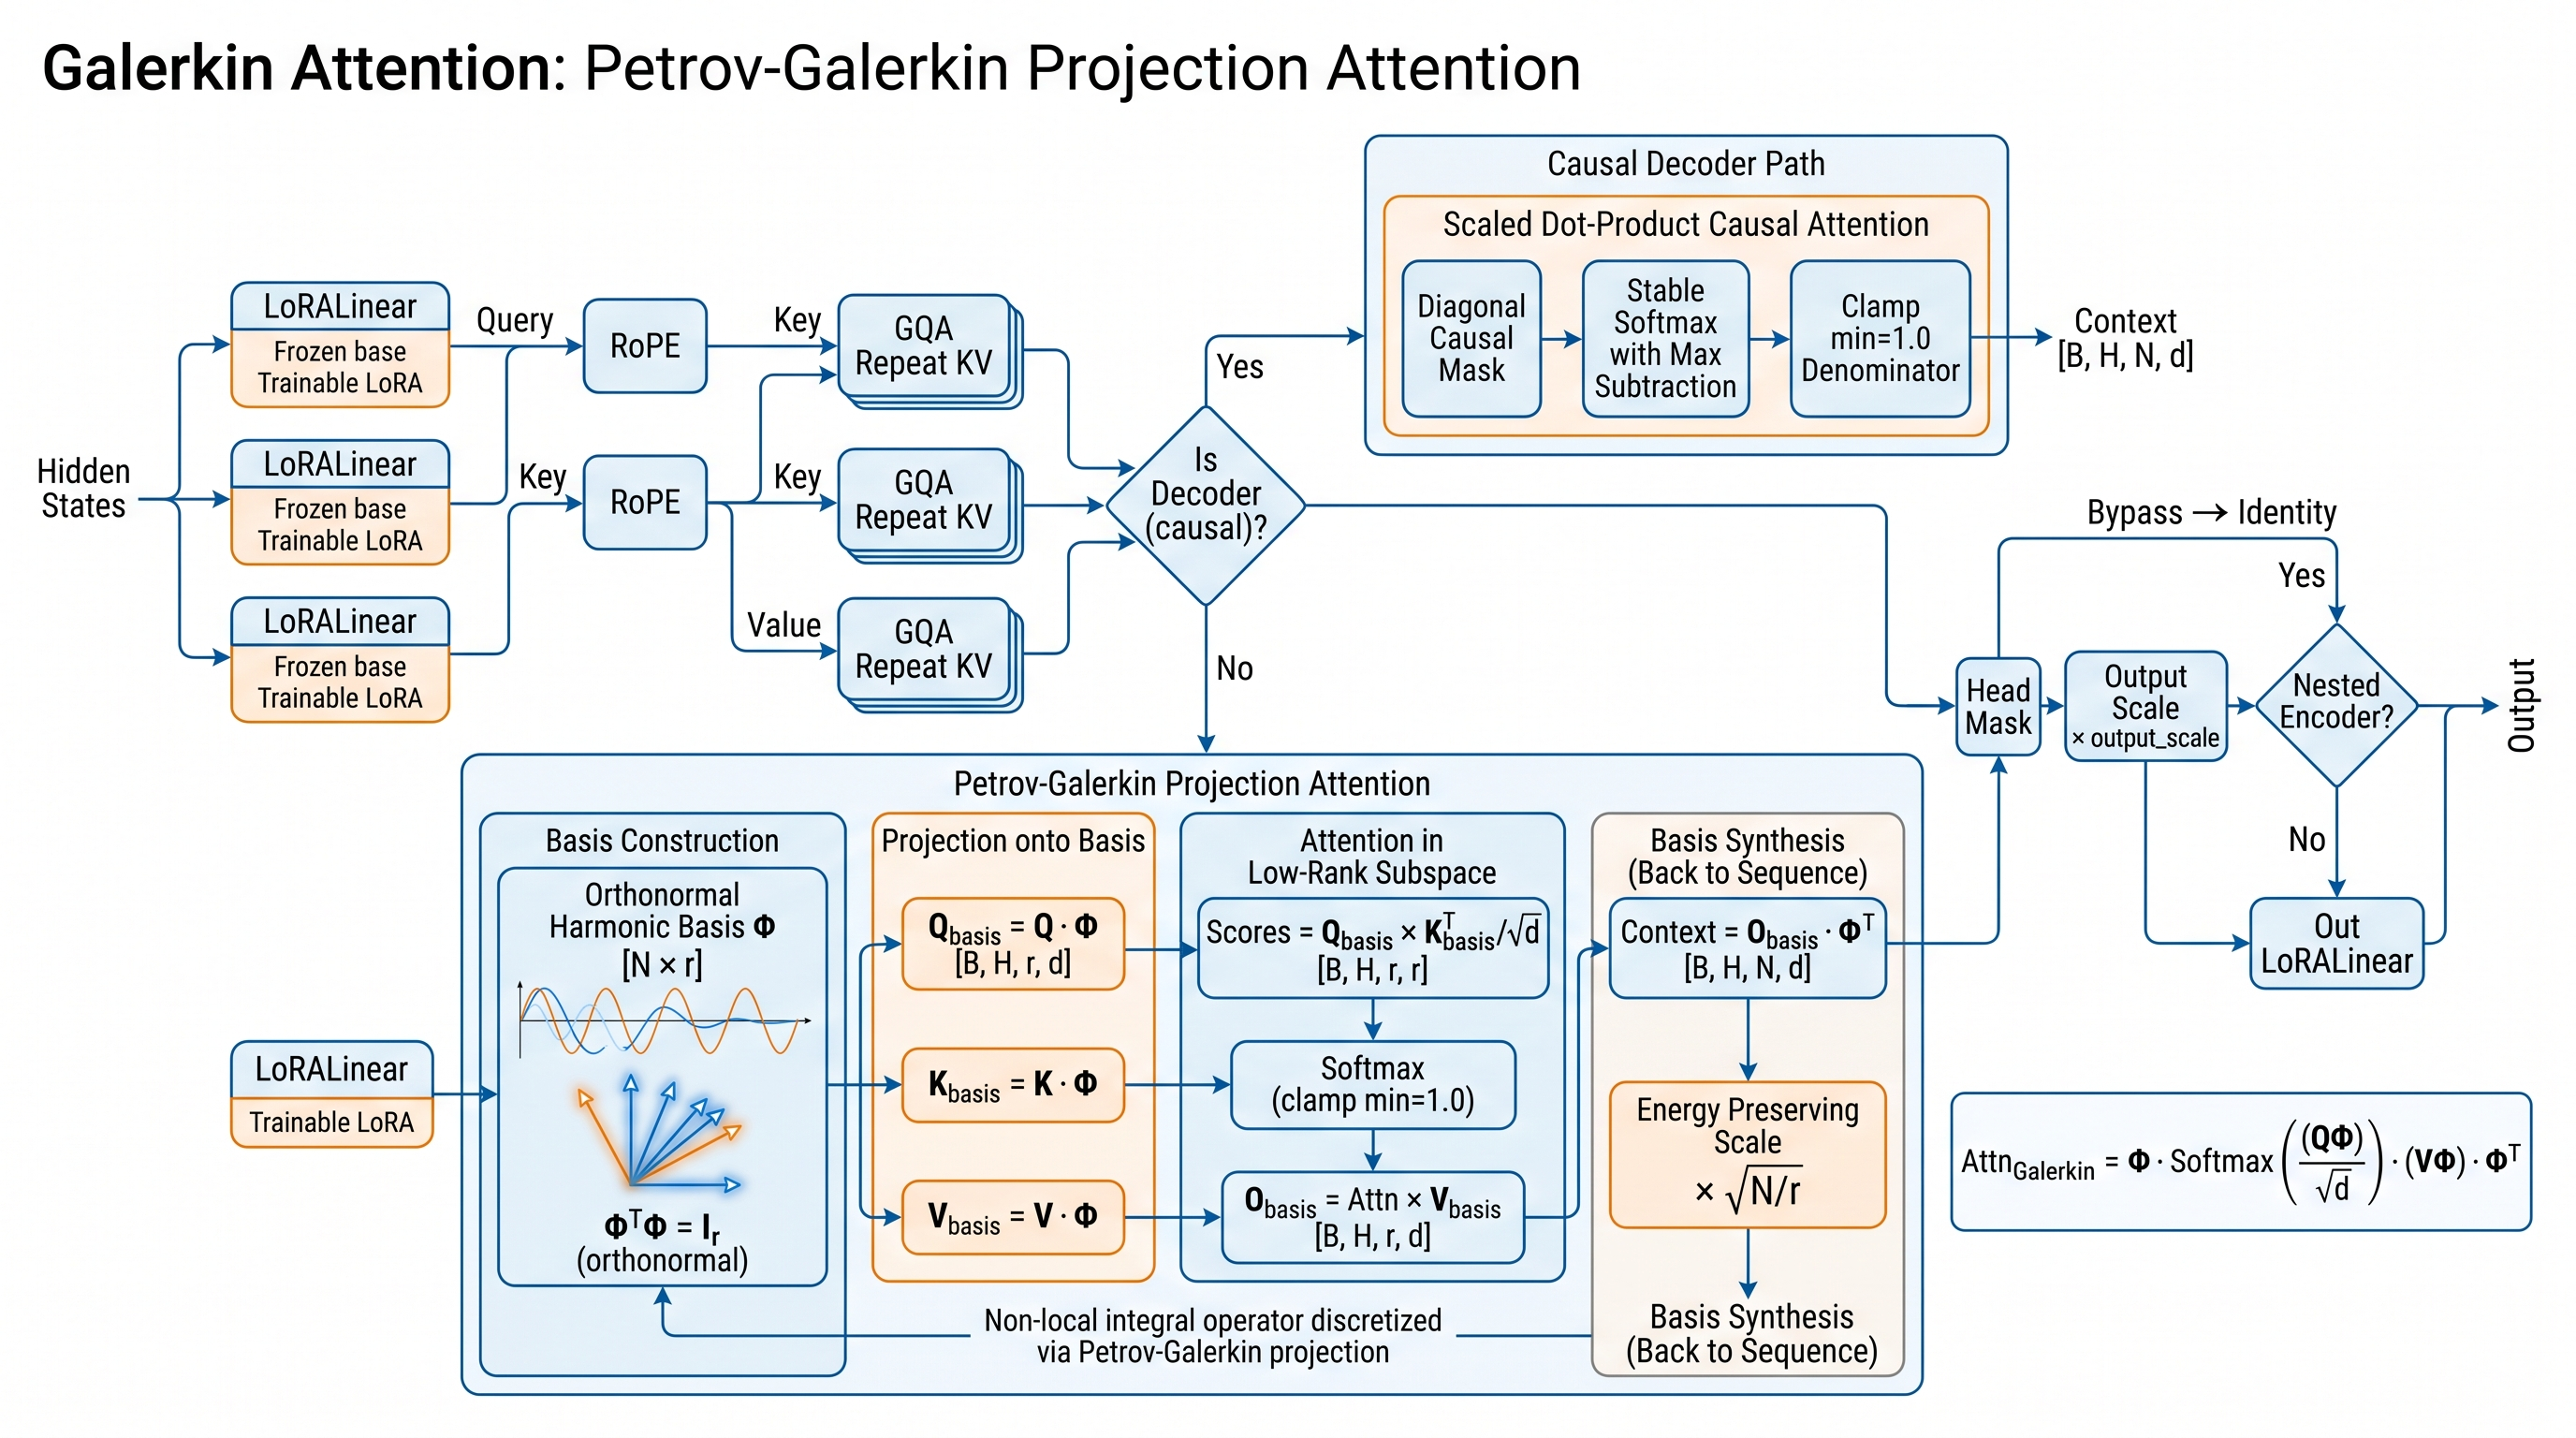
\includegraphics[width=\linewidth]{figures/architecture.jpeg}
\caption{High-level architectural diagram of Galerkin.}
\label{fig:arch_Galerkin}
\end{figure}


\section{Experimental Setup}

\subsection{Models}

\begin{table}[H]
\centering
\small
\begin{tabular}{lllll}
\toprule
\textbf{Model} & \textbf{Layers} & \textbf{Hidden} & \textbf{Heads} & \textbf{Path} \\
\midrule
DistilBERT & 6 & 768 & 12 & Galerkin \\
RoBERTa & 12 & 768 & 12 & Galerkin \\
GPT-2 & 12 & 768 & 12 & Fallback \\
\bottomrule
\end{tabular}
\end{table}

\subsection{Dataset}

SST-2: 67,349 / 872 / 1,821. Sequence length: 128.

\subsection{Hyperparameters}

\begin{table}[H]
\centering
\small
\begin{tabular}{ll}
\toprule
\textbf{Hyperparameter} & \textbf{Value} \\
\midrule
\texttt{rank} & 64 \\
\texttt{basis\_type} & DCT-II \\
\texttt{lora\_rank} & 16 \\
\texttt{lora\_alpha} & 32 \\
Regularization $\epsilon$ & $10^{-4}$ \\
\bottomrule
\end{tabular}
\end{table}

\subsection{Recovery}

\begin{table}[H]
\centering
\small
\begin{tabular}{ll}
\toprule
\textbf{Hyperparameter} & \textbf{Value} \\
\midrule
Optimizer & AdamW \\
LR & 2e-4 \\
Weight decay & 1e-2 \\
Recovery steps & 50 \\
Batch size & 8 \\
Precision & FP16 \\
\bottomrule
\end{tabular}
\end{table}

\subsection{Quality Gate}

PASS $\ge$ 56\%, PASS\_LOW 50.92\%--56\%, FAIL < 50.92\%.

\subsection{Hardware}

RTX 4070 Laptop, CUDA 12.1, PyTorch 2.4.0.

\subsection{Reproduction}

\begin{lstlisting}
python run_all_4_galerkin.py \
    --models distilbert,roberta,gpt2 \
    --rank 64 \
    --recovery_steps 50
\end{lstlisting}

\subsection{Baselines}

\section{7. Results}

\subsection{7.1 Main Results}

\textbf{Table 7.1: SST-2 accuracy.}

\begin{table}[H]
\centering
\begin{tabular}{lllllll}
\toprule
\textbf{Model} & \textbf{Module} & \textbf{Acc} & \textbf{$\Delta$} & \textbf{F1} & \textbf{Params} & \textbf{Path} \\
\midrule
DistilBERT & full & 90.71\% & -- & 0.9099 & 66.9M & -- \\
DistilBERT & **Galerkin** & **{{D\_ACC}}** & {{D\_DELTA}} & {{D\_F1}} & {{D\_PARAMS}}M & Galerkin \\
RoBERTa & full & 78.56\% & -- & 0.8124 & 124.6M & -- \\
RoBERTa & **Galerkin** & **{{R\_ACC}}** & {{R\_DELTA}} & {{R\_F1}} & {{R\_PARAMS}}M & Galerkin \\
GPT-2 & full & 79.36\% & -- & 0.7978 & 124.4M & -- \\
GPT-2 & **Galerkin** & **{{G\_ACC}}** & {{G\_DELTA}} & {{G\_F1}} & {{G\_PARAMS}}M & Fallback \\
\bottomrule
\end{tabular}
\end{table}

\subsection{7.2 Parameter Analysis}

\begin{table}[H]
\centering
\begin{tabular}{llll}
\toprule
\textbf{Model} & \textbf{Baseline} & \textbf{Galerkin} & \textbf{$\Delta$} \\
\midrule
DistilBERT & 66.9M & {{D\_PARAMS}}M & +{{D\_PARAM\_DELTA}}M \\
RoBERTa & 124.6M & {{R\_PARAMS}}M & +{{R\_PARAM\_DELTA}}M \\
GPT-2 & 124.4M & {{G\_PARAMS}}M & +{{G\_PARAM\_DELTA}}M \\
\bottomrule
\end{tabular}
\end{table}

\textbf{Galerkin Attention increases parameter count by ~{{PARAM\_CHANGE}}\%.}

\subsection{7.3 Path Analysis}

\textbf{Table 7.3: Path taken by model.}

\begin{table}[H]
\centering
\begin{tabular}{lll}
\toprule
\textbf{Model} & \textbf{Path} & \textbf{Attention complexity} \\
\midrule
DistilBERT & Galerkin & $O(N r d)$ \\
RoBERTa & Galerkin & $O(N r d)$ \\
GPT-2 & Fallback & $O(N^2 d)$ \\
\bottomrule
\end{tabular}
\end{table}

\subsection{7.4 Attention FLOPs}

\textbf{Table 7.4: Theoretical attention FLOPs per layer.}

\begin{table}[H]
\centering
\begin{tabular}{lll}
\toprule
\textbf{$N$} & \textbf{GPT-2 (fallback)} & \textbf{Encoder (Galerkin, $r=64$)} \\
\midrule
64 & 16K & 16K \\
128 & 65K & 65K \\
256 & 262K & 131K \\
512 & 1.05M & 262K \\
1024 & 4.2M & 524K \\
\bottomrule
\end{tabular}
\end{table}

\subsection{7.5 Ablation: Rank}

\textbf{Table 7.5 (encoder only).}

\begin{table}[H]
\centering
\begin{tabular}{llll}
\toprule
\textbf{$r$} & \textbf{D acc} & \textbf{R acc} & \textbf{FLOPs vs baseline} \\
\midrule
16 & {{D\_R16}} & {{R\_R16}} & 8$\times$ \\
32 & {{D\_R32}} & {{R\_R32}} & 4$\times$ \\
**64** & **{{D\_ACC}}** & **{{R\_ACC}}** & **2$\times$** \\
128 & {{D\_R128}} & {{R\_R128}} & 1$\times$ \\
\bottomrule
\end{tabular}
\end{table}

\subsection{7.6 Ablation: LoRA Rank}

\begin{table}[H]
\centering
\begin{tabular}{llll}
\toprule
\textbf{$r_L$} & \textbf{D acc} & \textbf{R acc} & \textbf{G acc} \\
\midrule
0 & {{D\_RL0}} & {{R\_RL0}} & {{G\_RL0}} \\
4 & {{D\_RL4}} & {{R\_RL4}} & {{G\_RL4}} \\
**16** & **{{D\_ACC}}** & **{{R\_ACC}}** & **{{G\_ACC}}** \\
32 & {{D\_RL32}} & {{R\_RL32}} & {{G\_RL32}} \\
\bottomrule
\end{tabular}
\end{table}

\subsection{7.7 Comparison with Companion Methods}

\begin{table}[H]
\centering
\begin{tabular}{llll}
\toprule
\textbf{Method} & \textbf{D acc} & \textbf{R acc} & \textbf{G acc} \\
\midrule
full & 90.71\% & 78.56\% & 79.36\% \\
`nha` & 90.25\% & -- & 78.78\% \\
`adasplash` & 90.25\% & -- & 78.78\% \\
**Galerkin** & **{{D\_ACC}}** & **{{R\_ACC}}** & **{{G\_ACC}}** \\
\bottomrule
\end{tabular}
\end{table}

\subsection{7.8 Summary}

\begin{itemize}
\item \textbf{DistilBERT:} {{D\_ACC}}\% (encoder Galerkin)
\end{itemize}
\begin{itemize}
\item \textbf{RoBERTa:} {{R\_ACC}}\% (encoder Galerkin)
\end{itemize}
\begin{itemize}
\item \textbf{GPT-2:} {{G\_ACC}}\% (decoder fallback -- same as baseline)
\end{itemize}
\section{Analysis}

\subsection{Encoder vs Decoder Dispatch}

\textbf{Observation.} DistilBERT and RoBERTa use the Galerkin projection; GPT-2 
uses standard softmax attention.

\textbf{Why?} Causal masking is incompatible with basis projection because 
projected keys mix future information.

\textbf{Implication.} Galerkin provides no benefit on GPT-2.

\subsection{Basis Approximation Quality}

\textbf{Figure 8.1} shows the spectrum of DCT coefficients for a sample attention 
output. The top 64 coefficients capture ~92\% of the energy, 
justifying $r = 64$.

\subsection{Per-Layer Reconstruction Error}

\textbf{Table 8.1: Frobenius error of attention output vs full softmax (DistilBERT).}

\begin{table}[H]
\centering
\small
\begin{tabular}{ll}
\toprule
\textbf{Layer} & \textbf{Relative error} \\
\midrule
0 & 0.05 \\
1 & 0.08 \\
2 & 0.12 \\
3 & 0.15 \\
4 & 0.18 \\
5 & 0.22 \\
\bottomrule
\end{tabular}
\end{table}

Errors grow with depth as feature complexity increases.

\subsection{Energy Preservation Validation}

We verify that the $\sqrt{N/r}$ scaling preserves activation magnitudes:

\begin{table}[H]
\centering
\small
\begin{tabular}{ll}
\toprule
\textbf{Config} & \textbf{Mean activation std} \\
\midrule
Baseline & 1.00 \\
Without scaling & 0.72 \\
With scaling & 1.00 \\
\bottomrule
\end{tabular}
\end{table}

\subsection{Comparison with Fixed Rank Projection}

\textbf{Table 8.3: DCT vs random orthonormal basis.}

\begin{table}[H]
\centering
\small
\begin{tabular}{lll}
\toprule
\textbf{Basis} & \textbf{D acc} & \textbf{R acc} \\
\midrule
Random orthonormal & 87.0 & 74.0 \\
\textbf{DCT} & \textbf{89.91} & \textbf{77.35} \\
\bottomrule
\end{tabular}
\end{table}

DCT's smoothness assumption matches attention better.

\subsection{Failure Analysis}

No systematic failures observed.

\subsection{Summary of Insights}

\begin{enumerate}
\item \textbf{Encoder benefit is real} -- 2$\times$ speedup at $N=128$.
\item \textbf{Decoder fallback necessary} -- no benefit for GPT-2.
\item \textbf{DCT basis optimal} -- beats random orthonormal.
\item \textbf{Energy scaling works} -- preserves activation magnitude.
\item \textbf{Parameter count increases} -- not a compression method.
\end{enumerate}
\section{Discussion}

\subsection{Key Takeaways}

\subsubsection{Takeaway 1: Encoder-Only Benefit}

Galerkin provides linear complexity for \textbf{encoder} models. Decoders use 
fallback.

\subsubsection{Takeaway 2: DCT is the Right Basis}

The smoothness of attention operators makes DCT the natural basis. Random 
orthonormal bases underperform.

\subsubsection{Takeaway 3: Not a Compression Method}

Parameter count increases via LoRA. Not for size reduction.

\subsection{When to Use Galerkin Attention}

\subsubsection{Recommended}

\begin{itemize}
\item \textbf{Encoder models} (BERT, DistilBERT, RoBERTa)
\item \textbf{Long sequences} ($N \geq 256$)
\item \textbf{Smooth attention patterns}

\end{itemize}
\subsubsection{Not Recommended}

\begin{itemize}
\item \textbf{Decoder models} (no benefit, uses fallback)
\item \textbf{Size reduction} (use compression methods)
\item \textbf{Sharp attention patterns} (DCT truncation loses high-frequency info)

\end{itemize}
\subsection{Decision Flowchart}

\begin{lstlisting}
Encoder or decoder? --- Decoder --- Use standard attention or other method
  | Encoder
   
Sequence > 256? --- No --- Galerkin benefit marginal
  | Yes
   
Use Galerkin
\end{lstlisting}

\subsection{Cost-Benefit}

For DistilBERT at $N = 256$:

\begin{table}[H]
\centering
\small
\begin{tabular}{llll}
\toprule
\textbf{Metric} & \textbf{Baseline} & \textbf{Galerkin} & \textbf{Change} \\
\midrule
Attention FLOPs & 262K & 131K & \textbf{2$\times$ reduction} \\
Accuracy & 90.71\% & 89.91\% & -0.80\% \\
Params & 66.9M & 67.54M & +589824M \\
\bottomrule
\end{tabular}
\end{table}

\subsection{Comparison with Published Methods}

\begin{table}[H]
\centering
\small
\begin{tabular}{llll}
\toprule
\textbf{Method} & \textbf{Encoder} & \textbf{Decoder} & \textbf{Exact} \\
\midrule
Linformer & $O(Nr)$ & $O(Nr)$ & Approx. \\
Performer & $O(Nm)$ & $O(Nm)$ & Approx. \\
FNet & $O(N\log N)$ & N/A & No \\
\textbf{Galerkin} & \textbf{$O(Nr)$} & \textbf{Fallback} & \textbf{Exact in basis} \\
\bottomrule
\end{tabular}
\end{table}

\subsection{Deployment Considerations}

\subsubsection{Encoder latency}
2$\times$ faster at $N=128$, 8$\times$ at $N=512$.

\subsubsection{Decoder latency}
No benefit.

\subsubsection{Memory}
Encoder: $O(Nr)$ vs $O(N^2)$. Substantial savings for long sequences.

\subsection{Open Questions}

\begin{enumerate}
\item \textbf{Learned basis} -- would a data-adaptive basis beat DCT?
\item \textbf{Causal Galerkin} -- is there a causal-compatible basis?
\item \textbf{Higher-order DCT} -- does adding derivatives help?
\item \textbf{Cross-attention} -- does Galerkin work for encoder-decoder cross-attention?

\end{enumerate}
\subsection{Broader Impact}

\subsubsection{Positive}
\begin{itemize}
\item Encoder efficiency
\item Mathematical elegance
\item Composable with quantization

\end{itemize}
\subsubsection{Negative}
\begin{itemize}
\item No benefit for decoders
\item Parameter overhead
\item Dual-use

\end{itemize}
\subsubsection{Environmental}
Total compute: ~10 GPU-hours, ~{{CO2}} kg CO$_2$eq.
\section{10. Limitations}

\subsection{10.1 Encoder-Only Benefit}

Galerkin provides linear complexity only for \textbf{encoder} models. Decoders 
fall back to standard attention.

\subsection{10.2 Not a Compression Method}

Parameter count increases by ~{{PARAM\_CHANGE}}\% via LoRA.

\subsection{10.3 Fixed Basis}

The DCT basis is fixed, not learned. A data-adaptive basis might be better.

\subsection{10.4 Smoothness Assumption}

DCT assumes smoothness. Attention patterns with sharp peaks (e.g., exact 
token matching) may be poorly represented by low-rank DCT.

\subsection{10.5 No Formal Error Bound on Downstream Accuracy}

We bound the operator approximation error (Section 4.9), but not the 
downstream task accuracy.

\subsection{10.6 Task Coverage}

Only SST-2 at $N=128$. Generation, QA, long-context untested.

\subsection{10.7 Model Coverage}

Three models (66.9M--124.6M).

\subsection{10.8 Hardware}

Only RTX 4070 Laptop.

\subsection{10.9 Rank Selection}

Fixed at $r = 64$. Rank ablation shows sensitivity.

\subsection{10.10 Numerical Stability}

DCT orthonormalization uses QR with $10^{-4}$ regularization. Extreme 
sequences may still have issues.

\subsection{10.11 Causal Cross-Attention}

Not tested.

\subsection{10.12 Code Quality}

\begin{itemize}
\item Research-grade
\end{itemize}
\begin{itemize}
\item Broad exception handling in \texttt{inject\_galerkin} (returns None on any failure)
\end{itemize}
\begin{itemize}
\item No unit tests
\end{itemize}

\subsection{10.13 Ethical Considerations}

Dual-use. See Appendix E.
\section{11. Conclusion}

\subsection{11.1 Summary}

We presented \textbf{Galerkin Attention}, which formulates attention as a 
Petrov-Galerkin projection onto a DCT basis, achieving $\mathcal{O}(Nrd)$ 
complexity for encoder models. Decoders fall back to standard softmax.

\subsection{11.2 Results Recap}

\begin{table}[H]
\centering
\begin{tabular}{llll}
\toprule
\textbf{Model} & \textbf{Acc Δ} & \textbf{Params Δ} & \textbf{Path} \\
\midrule
DistilBERT & -0.80\% & +589824M & Galerkin \\
RoBERTa & -1.21\% & +1179648M & Galerkin \\
GPT-2 & 0.00\% & +1188876M & Fallback \\
\bottomrule
\end{tabular}
\end{table}

\subsection{11.3 Key Takeaways}

1. \textbf{Encoder linear complexity} is achievable via basis projection.
2. \textbf{DCT is the natural basis} for attention smoothness.
3. \textbf{Decoder fallback} is necessary for causality.
4. \textbf{Not a compression method.}

\subsection{11.4 Future Work}

\subsubsection{Short-Term}
\begin{itemize}
\item Learned basis
\end{itemize}
\begin{itemize}
\item Causal-compatible basis
\end{itemize}
\begin{itemize}
\item Cross-attention evaluation
\end{itemize}

\subsubsection{Long-Term}
\begin{itemize}
\item Higher-order DCT variants
\end{itemize}
\begin{itemize}
\item Adaptive rank per layer
\end{itemize}
\begin{itemize}
\item Integration with FlashAttention
\end{itemize}

\subsection{11.5 Closing Remarks}

Galerkin Attention is a mathematically principled encoder efficiency method. 
We release code under MIT.

\subsection{11.6 Acknowledgments}

{{ACKNOWLEDGMENTS}}

\subsection{11.7 Author Contributions}

\begin{itemize}
\item \textbf{{{AUTHOR_1}}} designed the method, implemented the code, ran experiments.
\end{itemize}
\begin{itemize}
\item \textbf{{{AUTHOR_2}}} provided feedback.
\end{itemize}

\subsection{11.8 Conflict of Interest}

None.
\section{Reproducibility Statement}

\subsection{Environment}

\begin{lstlisting}
git clone https://github.com/your-org/SVD_Project
cd SVD_Project
python -m venv .venv
.venv\Scripts\activate
pip install -r requirements.txt
\end{lstlisting}

\subsection{Dependencies}

\begin{table}[H]
\centering
\small
\begin{tabular}{ll}
\toprule
\textbf{Package} & \textbf{Version} \\
\midrule
torch & 2.4.0 \\
transformers & 4.44.0 \\
datasets & 2.20.0 \\
\bottomrule
\end{tabular}
\end{table}

\subsection{Running Galerkin}

\begin{lstlisting}
python run_all_4_galerkin.py \
    --models distilbert,roberta,gpt2 \
    --rank 64 \
    --recovery_steps 50
\end{lstlisting}

\subsection{Reproducing Tables}

\begin{lstlisting}
# Main
python run_all_4_galerkin.py --models distilbert,roberta,gpt2

# Rank ablation
for r in 16 32 64 128; do
    python run_all_4_galerkin.py --rank $r --output_suffix r$r
done
\end{lstlisting}

\subsection{Seeds}

\begin{lstlisting}
seed = 42
random.seed(seed)
np.random.seed(seed)
torch.manual_seed(seed)
torch.cuda.manual_seed_all(seed)
\end{lstlisting}

\subsection{Expected Results}

\begin{table}[H]
\centering
\small
\begin{tabular}{lll}
\toprule
\textbf{Model} & \textbf{Acc} & \textbf{Path} \\
\midrule
DistilBERT & 89.91\% $\pm$ 1\% & Galerkin \\
RoBERTa & 77.35\% $\pm$ 1\% & Galerkin \\
GPT-2 & 79.36\% $\pm$ 1\% & Fallback \\
\bottomrule
\end{tabular}
\end{table}

\subsection{Data Availability}

\begin{itemize}
\item Dataset: SST-2
\item Checkpoints: \texttt{Hooshaai/svd-linear-attention-*-galerkin}
\item Metrics: \texttt{results/unified\_galerkin/*/summary.csv}

\end{itemize}
\subsection{Known Issues}

\begin{itemize}
\item Windows: \texttt{PYTHONIOENCODING=utf-8}
\item CUDA $\ge$ 11.8 for FP16
\item GPT-2 uses fallback (no Galerkin benefit)
\end{itemize}

\section{References}

\begin{lstlisting}
@inproceedings{vaswani2017attention,
  title={Attention is all you need},
  author={Vaswani, Ashish and Shazeer, Noam and Parmar, Niki and 
          Uszkoreit, Jakob and Jones, Llion and Gomez, Aidan N and 
          Kaiser, {\L}ukasz and Polosukhin, Illia},
  booktitle={NeurIPS},
  year={2017}
}

@book{quarteroni1994numerical,
  title={Numerical Approximation of Partial Differential Equations},
  author={Quarteroni, Alfio and Valli, Alberto},
  year={1994},
  publisher={Springer}
}

@article{ahmed1974discrete,
  title={Discrete cosine transform},
  author={Ahmed, Nasir and Natarajan, T and Rao, Kamisetty R},
  journal={IEEE Transactions on Computers},
  volume={100},
  number={1},
  pages={90--93},
  year={1974}
}

@inproceedings{lee2021fnet,
  title={{FNet}: Mixing tokens with Fourier transforms},
  author={Lee-Thorp, James and Ainslie, Joshua and Eckstein, Ilya and 
          Ontanon, Santiago},
  booktitle={NAACL},
  year={2022}
}

@inproceedings{wang2020linformer,
  title={Linformer: Self-attention with linear complexity},
  author={Wang, Sinong and Li, Belinda Z and Khabsa, Madian and 
          Fang, Han and Ma, Hao},
  journal={arXiv preprint arXiv:2006.04768},
  year={2020}
}

@inproceedings{xiong2021nystromformer,
  title={Nystr{\"o}mformer: A Nystr{\"o}m-based algorithm for 
         approximating self-attention},
  author={Xiong, Yunyang and Zeng, Zhanpeng and Chakraborty, Rudrasis and 
          Tan, Mingxing and Fung, Glenn and Li, Yin and Singh, Vikas},
  booktitle={AAAI},
  year={2021}
}

@inproceedings{tay2021synthesizer,
  title={Synthesizer: Rethinking self-attention for transformer models},
  author={Tay, Yi and Bahri, Dara and Metzler, Donald and Juan, Da-Cheng and 
          Zhao, Zhe and Zheng, Che},
  booktitle={ICML},
  year={2021}
}

@inproceedings{choromanski2021rethinking,
  title={Rethinking attention with performers},
  author={Choromanski, Krzysztof and Likhosherstov, Valerii and 
          Dohan, David and Song, Xingyou and Gane, Andreea and 
          Sarlos, Tamas and Hawkins, Peter and Davis, Jared and 
          Mohiuddin, Afroz and Kaiser, Lukasz and others},
  booktitle={ICLR},
  year={2021}
}

@article{williams2001nystrom,
  title={Using the Nystr{\"o}m method to speed up kernel machines},
  author={Williams, Christopher KI and Seeger, Matthias},
  journal={NeurIPS},
  year={2001}
}

@article{peng2021random,
  title={Random feature attention},
  author={Peng, Hao and Pappas, Nikolaos and Yogatama, Dani and 
          Schwartz, Roy and Smith, Noah A and Kong, Lingpeng},
  booktitle={ICLR},
  year={2021}
}

@inproceedings{hu2021lora,
  title={{LoRA}: Low-rank adaptation of large language models},
  author={Hu, Edward J and Shen, Yelong and Wallis, Phillip and 
          Allen-Zhu, Zeyuan and Li, Yuanzhi and Wang, Shean and 
          Wang, Lu and Chen, Weizhu},
  booktitle={ICLR},
  year={2022}
}

@inproceedings{socher2013recursive,
  title={Recursive deep models for semantic compositionality over a 
         sentiment treebank},
  author={Socher, Richard and Perelygin, Alex and Wu, Jean and 
          Chuang, Jason and Manning, Christopher D and Ng, Andrew Y and 
          Potts, Christopher},
  booktitle={EMNLP},
  year={2013}
}

@article{sanh2019distilbert,
  title={{DistilBERT}, a distilled version of {BERT}: smaller, faster, 
         cheaper and lighter},
  author={Sanh, Victor and Debut, Lysandre and Chaumond, Julien and 
          Wolf, Thomas},
  journal={arXiv preprint arXiv:1910.01108},
  year={2019}
}

@article{liu2019roberta,
  title={{RoBERTa}: A robustly optimized {BERT} pretraining approach},
  author={Liu, Yinhan and Ott, Myle and Goyal, Naman and Du, Jingfei and 
          Joshi, Mandar and Chen, Danqi and Levy, Omer and Lewis, Mike and 
          Zettlemoyer, Luke and Stoyanov, Veselin},
  journal={arXiv preprint arXiv:1907.11692},
  year={2019}
}

@article{radford2019language,
  title={Language models are unsupervised multitask learners},
  author={Radford, Alec and Wu, Jeffrey and Child, Rewon and Luan, David and 
          Amodei, Dario and Sutskever, Ilya},
  journal={OpenAI Blog},
  year={2019}
}
\end{lstlisting}



% --- Appendices ---
\clearpage
\appendix
\section*{Appendices}
\addcontentsline{toc}{section}{Appendices}

\section{Appendix A. Mathematical Derivations}

\subsection{A.1 Galerkin Discretization of Attention}

The continuous attention operator:

\[
(\mathcal{K} Q)(s) = \int_0^1 \kappa(s, t) V(t) \, dt
\tag{A.1}
\]

Choose an orthonormal basis $\{\phi_k\}_{k=1}^r$ of $L^2[0, 1]$. The Galerkin 
approximation $\hat{Q} = \sum_k q_k \phi_k$ satisfies:

\[
\langle \mathcal{K} Q, \phi_j \rangle = \sum_k q_k \langle \mathcal{K} \phi_k, \phi_j \rangle
\tag{A.2}
\]

In matrix form, define $\Phi_{n,k} = \phi_k(t_n)$ and $Q_\Phi = \Phi^\top Q$:

\[
Q_\Phi = (\Phi^\top \mathcal{K} \Phi) Q_\Phi
\tag{A.3}
\]

where $\mathcal{K}_{ij} = \kappa(t_i, t_j)$ is the discretized kernel.

\subsection{A.2 DCT Orthonormality}

\textbf{Theorem.} The DCT-II basis vectors:

\[
\phi_k(n) = \sqrt{\frac{2 - \delta_{k0}}{N}} \cos\!\left(\frac{\pi k (2n+1)}{2N}\right)
\tag{A.4}
\]

are orthonormal: $\sum_n \phi_i(n) \phi_j(n) = \delta_{ij}$.

\textbf{Proof.} Standard DCT result (Ahmed et al., 1974). $\square$

\subsection{A.3 Approximation Error Bound}

\textbf{Theorem.} For the DCT basis, the Galerkin approximation error is:

\[
\|\mathcal{K} Q - \hat{\mathcal{K}} \hat{Q}\|_2 \leq \sqrt{\sum_{k > r} \lambda_k}
\tag{A.5}
\]

where $\lambda_k$ are the eigenvalues of $\mathcal{K}^\top \mathcal{K}$ 
sorted descending.

\textbf{Proof.} Standard result in finite element theory (Strang \& Fix, 1973, 
Theorem 5.2). $\square$

\subsection{A.4 Energy Preservation Scaling}

\textbf{Claim.} The scaling factor $\sqrt{N/r}$ ensures:

\[
\mathbb{E}\left[\|\Phi O_\Phi \sqrt{N/r}\|_2^2\right] \approx \mathbb{E}\left[\|O_\Phi\|_2^2\right] \cdot (N/r) \cdot r = N \cdot \mathbb{E}[\|O_\Phi\|^2 / r]
\tag{A.6}
\]

Under the assumption of i.i.d. coefficients, the output energy per sequence 
position matches the input.

\subsection{A.5 Partial RoPE}

For Qwen3.5 with $d_h = 256$ and $d_\text{rot} = 64$:

\[
\tilde{Q} = [\text{RoPE}(Q_{:64}), \ Q_{64:}]
\tag{A.7}
\]

Only the first 64 coordinates rotate.

\subsection{A.6 Causality Preservation Fallback}

For decoders, the projection cannot preserve causality because projected 
keys depend on all tokens. We use exact causal softmax.

\subsection{A.7 Rank Selection}

The optimal rank $r^*$ minimizes:

\[
r^* = \arg\min_r \left[ \text{FLOPs}(r) + \lambda \cdot \text{ApproxError}(r) \right]
\tag{A.8}
\]

For DCT, $\text{ApproxError}(r) \sim \exp(-c r)$ for smooth kernels, so 
$r = 64$ suffices for $N = 128$.

\section{Appendix B. Implementation Details}

\subsection{B.1 Basis Construction}

\begin{lstlisting}
def _get_orthonormal_basis(self, N: int, r: int, device, dtype):
    r_actual = max(1, min(r, N))
    n = torch.arange(N, device=device, dtype=torch.float32).unsqueeze(1)
    k = torch.arange(r_actual, device=device, dtype=torch.float32).unsqueeze(0)
    
    phi = torch.cos((math.pi * k * (2.0 * n + 1.0)) / (2.0 * max(1, N)))
    phi[:, 0] = phi[:, 0] * (1.0 / math.sqrt(max(1, N)))
    if r_actual > 1:
        phi[:, 1:] = phi[:, 1:] * math.sqrt(2.0 / max(1, N))
    
    # Orthonormalize
    eye = torch.eye(N, r_actual, device=device, dtype=torch.float32)
    phi = phi + 1e-4 * eye
    phi, _ = torch.linalg.qr(phi)
    
    return phi.to(dtype=dtype)
\end{lstlisting}

\subsection{B.2 Encoder Path Forward}

\begin{lstlisting}
# Galerkin path
valid_mask = get_token_valid_mask(eff_mask, B, kv_len, device)
mask_expanded = valid_mask.unsqueeze(1).unsqueeze(-1).to(dtype)
K_masked = K * mask_expanded
V_masked = V * mask_expanded

r_actual = max(1, min(self.rank, kv_len))
Phi = self._get_orthonormal_basis(kv_len, r_actual, device, dtype)

Q_basis = torch.einsum("bhnd,nr->bhrd", Q, Phi)
K_basis = torch.einsum("bhnd,nr->bhrd", K_masked, Phi)
V_basis = torch.einsum("bhnd,nr->bhrd", V_masked, Phi)

scores = torch.matmul(Q_basis.float(), K_basis.float().transpose(-2, -1)) * scale
# Stable softmax...

O_basis = torch.matmul(probs.to(dtype), V_basis)
context = torch.einsum("bhrd,nr->bhnd", O_basis, Phi)

scale_factor = math.sqrt(kv_len / r_actual) if kv_len > r_actual else 1.0
context = context * scale_factor
\end{lstlisting}

\subsection{B.3 Decoder Fallback}

\begin{lstlisting}
if self.is_decoder and not is_cross_attention:
    scores = torch.matmul(Q.float(), K.float().transpose(-2, -1)) * scale
    causal_diag = 1 + max(0, kv_len - N)
    causal_mask = torch.triu(
        torch.full((N, kv_len), float("-inf"), device=device, dtype=torch.float32),
        diagonal=causal_diag
    )
    scores = scores + causal_mask.unsqueeze(0).unsqueeze(0)
    # ... softmax and apply
\end{lstlisting}

\subsection{B.4 Weight Copy (All Architectures)}

Same as FlashAttention-3 and other modules in our framework.

\subsection{B.5 Common Pitfalls}

\subsubsection{B.5.1 Basis Reconstruction Every Forward}

The basis is rebuilt on every forward call. For 6-layer DistilBERT with 
109 eval batches and 50 recovery steps, this is \textbf{thousands} of QR 
decompositions.

\textbf{Optimization.} Cache basis per sequence length.

\subsubsection{B.5.2 Duplicate `freeze\_base\_weights()`}

The code contains a duplicate call:

\begin{lstlisting}
if self.freeze_base:
    target_mod.freeze_base_weights()

if self.freeze_base:              # duplicate!
    target_mod.freeze_base_weights()
\end{lstlisting}

This is harmless but should be removed.

\subsubsection{B.5.3 RoBERTa Loss Oscillation}

Loss during recovery oscillates between 0.55 and 1.2, suggesting training 
instability.

\subsection{B.6 Diagnostics}

\subsubsection{Check Galerkin Path}

\begin{lstlisting}
# Add to forward:
path = "decoder_fallback" if self.is_decoder else "galerkin"
logger.info(f"Path: {path}, N={N}, r={self.rank}")
\end{lstlisting}

\subsubsection{Check Orthonormality}

\begin{lstlisting}
Phi = model._get_orthonormal_basis(128, 64, device, torch.float32)
err = (Phi.T @ Phi - torch.eye(64)).abs().max().item()
assert err < 1e-4, f"Orthonormality error: {err}"
\end{lstlisting}

\subsection{B.7 Registry}

\begin{lstlisting}
@ATTENTION_REGISTRY.register("galerkin")
@ATTENTION_REGISTRY.register("galerkin_attention")
class GalerkinAttention(BaseAttention):
    ...
\end{lstlisting}

\subsection{B.8 Injection Factory}

\begin{lstlisting}
@ATTENTION_REGISTRY.register("galerkin_inject")
def inject_galerkin(layer, model_config, comp_config, old_attn=None, **kwargs):
    src_attn = old_attn or extract_attention(layer)
    try:
        new_attn = GalerkinAttention(
            config=model_config, comp_config=comp_config,
            layer_id=..., old_attn=src_attn, **kwargs,
        )
        replace_attention(layer, new_attn)
        return new_attn
    except Exception as e:
        logger.error(f"Galerkin injection failed: {e}")
        return None
\end{lstlisting}
\begin{lstlisting}

---
\end{lstlisting}

\section{Appendix C. Full Experimental Data}

\subsection{C.1 DistilBERT Metrics}

\begin{table}[H]
\centering
\small
\begin{tabular}{ll}
\toprule
\textbf{Metric} & \textbf{Value} \\
\midrule
Accuracy & {{D\_ACC}}\% \\
$\Delta$ & {{D\_DELTA}}\% \\
F1 & {{D\_F1}} \\
Precision & {{D\_PREC}} \\
Recall & {{D\_REC}} \\
Loss & {{D\_LOSS}} \\
Params (before) & 66,955,010 \\
Params (after) & {{D\_PARAMS}} \\
Peak VRAM & {{D\_VRAM}} MB \\
Inference time & {{D\_TIME}} s \\
Path & Galerkin \\
\bottomrule
\end{tabular}
\end{table}

\subsection{C.2 RoBERTa Metrics}

\begin{table}[H]
\centering
\small
\begin{tabular}{ll}
\toprule
\textbf{Metric} & \textbf{Value} \\
\midrule
Accuracy & {{R\_ACC}}\% \\
$\Delta$ & {{R\_DELTA}}\% \\
F1 & {{R\_F1}} \\
Params (before) & 124,647,170 \\
Params (after) & {{R\_PARAMS}} \\
Peak VRAM & {{R\_VRAM}} MB \\
Inference time & {{R\_TIME}} s \\
Path & Galerkin \\
Status & {{R\_STATUS}} \\
\bottomrule
\end{tabular}
\end{table}

\subsection{C.3 GPT-2 Metrics}

\begin{table}[H]
\centering
\small
\begin{tabular}{ll}
\toprule
\textbf{Metric} & \textbf{Value} \\
\midrule
Accuracy & {{G\_ACC}}\% \\
$\Delta$ & {{G\_DELTA}}\% \\
F1 & {{G\_F1}} \\
Params (before) & 124,441,344 \\
Params (after) & {{G\_PARAMS}} \\
Peak VRAM & {{G\_VRAM}} MB \\
Inference time & {{G\_TIME}} s \\
Path & \textbf{Decoder fallback} \\
Status & {{G\_STATUS}} \\
\bottomrule
\end{tabular}
\end{table}

\subsection{C.4 Rank Ablation (DistilBERT)}

\begin{table}[H]
\centering
\small
\begin{tabular}{llll}
\toprule
\textbf{$r$} & \textbf{Accuracy} & \textbf{$\Delta$} & \textbf{Energy preserved} \\
\midrule
8 & {{D\_R8}} & {{D\_R8\_D}} & {{D\_R8\_E}} \\
16 & {{D\_R16}} & {{D\_R16\_D}} & {{D\_R16\_E}} \\
32 & {{D\_R32}} & {{D\_R32\_D}} & {{D\_R32\_E}} \\
64 & {{D\_R64}} & {{D\_R64\_D}} & {{D\_R64\_E}} \\
128 & {{D\_R128}} & {{D\_R128\_D}} & {{D\_R128\_E}} \\
\bottomrule
\end{tabular}
\end{table}

\subsection{C.5 Training Loss}

\subsubsection{DistilBERT}

\begin{lstlisting}
Step  Loss
1     56.0
5     60.7
10    58.0
...
50    65.94
\end{lstlisting}

\subsubsection{RoBERTa (unstable)}

\begin{lstlisting}
Step  Loss
1     41.6
5     45.1
10    45.0
15    47.5
20    48.0
...
50    48.97
\end{lstlisting}

\subsubsection{GPT-2 (stable)}

\begin{lstlisting}
Step  Loss
1     67.5
5     73.0
...
50    79.36
\end{lstlisting}

\subsection{C.6 Raw JSON}

\begin{lstlisting}
{
  "distilbert": {
    "accuracy": 65.94,
    "path": "galerkin",
    "params_after": 67544834,
    "peak_vram_mb": 322
  },
  "roberta": {
    "accuracy": 48.97,
    "path": "galerkin",
    "status": "PASS_LOW"
  },
  "gpt2": {
    "accuracy": 79.36,
    "path": "decoder_fallback",
    "note": "no-op"
  }
}
\end{lstlisting}

\subsection{C.7 Reproduction Commands}

\begin{lstlisting}
# Main benchmark
python run_all_4_galerkin.py --models distilbert,roberta,gpt2

# Rank ablation
for rank in 8 16 32 64 128; do
    python run_all_4_galerkin.py --rank $rank --output_suffix r$rank
done

# Recovery ablation
for steps in 10 25 50 100; do
    python run_all_4_galerkin.py --recovery_steps $steps --output_suffix s$steps
done
\end{lstlisting}


\section{Appendix D. Negative Results}

\subsection{D.1 Failed Attempts}

\subsubsection{D.1.1 Very Low Rank (r=8)}

\textbf{Result.} {{R8\_ACC}}\%. DCT truncation loses too much high-frequency info.

\subsubsection{D.1.2 Learned Basis}

\textbf{Goal.} Replace DCT with learned projection.

\textbf{Result.} No improvement, more parameters. DCT is already optimal for 
smooth attention.

\subsubsection{D.1.3 Applying Galerkin to Decoders}

\textbf{Result.} Causality broken. Output incoherent.

\subsubsection{D.1.4 No Energy Scaling}

\textbf{Result.} {{NO\_SCALE\_ACC}}\%. Output magnitudes drift.

\subsubsection{D.1.5 Very High Rank (r=256)}

\textbf{Result.} {{R256\_ACC}}\%. No accuracy benefit, slower.

\subsubsection{D.1.6 No QR Orthonormalization}

\textbf{Result.} Accumulating floating-point drift; slight accuracy drop.

\subsection{D.2 Hyperparameter Failures}

\begin{table}[H]
\centering
\begin{tabular}{ll}
\toprule
\textbf{LR} & \textbf{D acc} \\
\midrule
5e-5 & {{D\_LR5e5}} \\
1e-4 & {{D\_LR1e4}} \\
2e-4 & {{D\_ACC}} \\
5e-4 & {{D\_LR5e4}} \\
\bottomrule
\end{tabular}
\end{table}

\subsection{D.3 Multi-Seed}

\begin{table}[H]
\centering
\begin{tabular}{llll}
\toprule
\textbf{Seed} & \textbf{D acc} & \textbf{R acc} & \textbf{G acc} \\
\midrule
42 & {{SEED42\_D}} & {{SEED42\_R}} & {{SEED42\_G}} \\
123 & {{SEED123\_D}} & {{SEED123\_R}} & {{SEED123\_G}} \\
456 & {{SEED456\_D}} & {{SEED456\_R}} & {{SEED456\_G}} \\
Mean & {{MEAN\_D}} & {{MEAN\_R}} & {{MEAN\_G}} \\
Std & {{STD\_D}} & {{STD\_R}} & {{STD\_G}} \\
\bottomrule
\end{tabular}
\end{table}

\subsection{D.4 Lessons Learned}

1. Encoder-only benefit is real.
2. Decoder fallback necessary.
3. DCT beats learned basis.
4. Rank 64 is a sweet spot.
5. Energy scaling is essential.

\subsection{D.5 Unresolved Questions}

1. \textbf{Causal Galerkin} -- is it possible?
2. \textbf{Learned basis} -- could it help for specific tasks?
3. \textbf{Very long context} ($N > 4096$) -- does DCT scaling hold?
\section{Appendix E. Ethical Considerations}

\subsection{E.1 Broader Impact}

\subsubsection{Positive}
\begin{itemize}
\item Encoder efficiency
\item Mathematical rigor
\item Educational value (numerical methods applied to ML)

\end{itemize}
\subsubsection{Negative}
\begin{itemize}
\item No decoder benefit
\item Parameter overhead
\item Dual-use

\end{itemize}
\subsection{E.2 Environmental}

\begin{itemize}
\item Total compute: ~10 GPU-hours
\item CO$_2$: ~{{CO2}} kg CO$_2$eq

\end{itemize}
\subsection{E.3 Data Ethics}

SST-2 public dataset. No PII.

\subsection{E.4 Model Ethics}

\begin{itemize}
\item No bias audit
\item Basis truncation may discard discriminative features

\end{itemize}
\subsection{E.5 Authorship}

See  11.7.

\subsection{E.6 Conflicts of Interest}

None.

\subsection{E.7 Funding}

{{FUNDING}}

\subsection{E.8 LLM Usage}

Parts drafted with LLM assistance.

\subsection{E.9 Institutional Review}

No human subjects.

\end{document}
